
\documentclass[11pt]{article} 

\usepackage[utf8]{inputenc} 
\usepackage{geometry} 
\geometry{a4paper} 

\vspace{2cm}
\setlength{\parindent}{0cm}
\usepackage{graphicx,wrapfig,placeins}

\title{Disney BRDF}
\author{Chichi Francesco}

\begin{document}
\maketitle
\graphicspath{{img/}}
\section{Introduction}
	The project developed aims to implement the The bidirectional reflectance distribution function .
\section{Other libraries}
\begin{itemize}
	\item \textbf{yocto-gl:}
		Yocto/GL is a collection utilities for building physically-based graphics algorithms implemented as a two-file library, and released under the MIT license.
		
\end{itemize}

\newpage
\section{Bidirectional reflectance distribution function (BRDF)}
The bidirectional reflectance distribution function is a function $ f(x,i,o) $ that defines how light is reflected at an opaque surface (figure \ref{fig:reflect}), and is defined as the ratio of the differential reflected radiance over the
differential incident irradiance. 
In simple terms, the BRDF define the probability that a photon coming from a direction \textit{i} is reflected in a direction \textit{r}, after the collision with an opaque surface.
We can so define it as \cite{slide}:
$f(x,i,o)=\frac{\delta L_r(x,o)}{\delta E_i(x,i)} = \frac{\delta L_r(x,o)}{L_i(x,i)(n_x\cdot i) \delta \omega_i} $

\begin{figure}
	\centering
	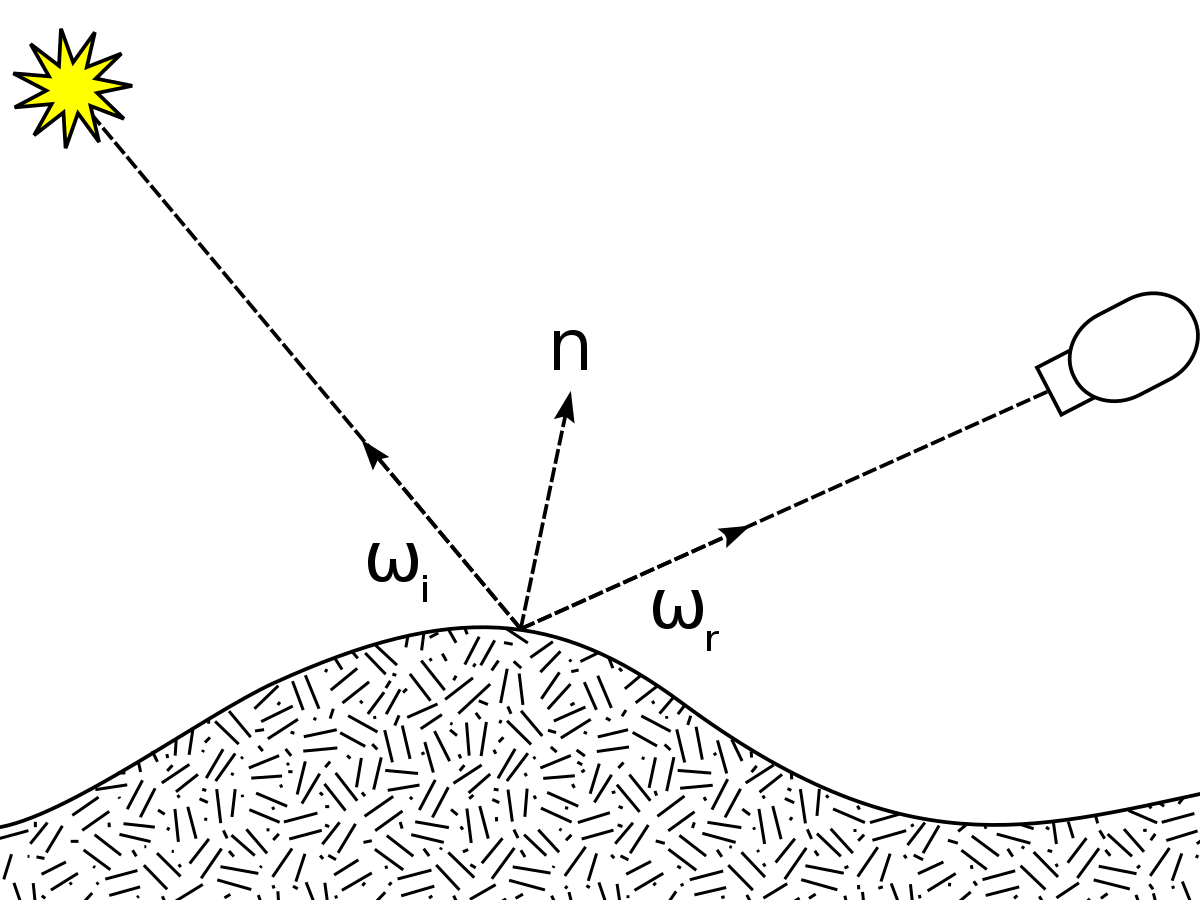
\includegraphics[width=0.5\linewidth]{img/reflect}
	\caption{A graphical example of the photon's reflection on an opaque surface.}
	\label{fig:reflect}
\end{figure}

A physically based specular BRDF is based on micro-facet theory, which describe a surface is composed of many micro-facets and each micro-facet will only reflect light in a single direction according to their normal(m) (figure \ref{fig:microfacet}) \cite{slide,microfacet} 

\begin{figure}
	\centering
	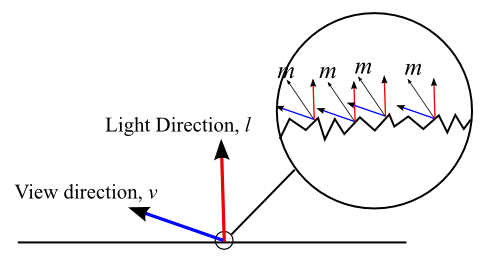
\includegraphics[width=0.5\linewidth]{img/microfacet}
	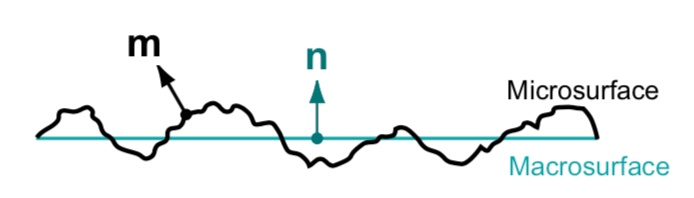
\includegraphics[width=0.5\linewidth]{img/microfacet2}
	\caption{A graphical example of the photon's reflection on the microfacets surfaces.}
	\label{fig:microfacet}
\end{figure}

So, the BRDF is essentially the "average" value of all these reflection events among all the micro-facets.
The microfacet reflection is then the normalized product of three terms:
$f_r(i,o)=\frac{F(i,h)D(h)G(h,i,o)}{4|n\cdot i||n\cdot o|}$\\
$h= \frac{i+o}{|i+o|}$ \\
Where F is the fresnel term, that take accounts for difference at grazing angle, the microfacet distribution D describes the statistical distribution of microfacets in a surface and the shadow-masking term G, that corrects for facets not visible from light or from the point of view (fig \ref{fig:visible})

\begin{figure}
	\centering
	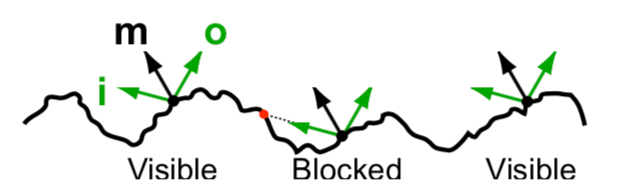
\includegraphics[width=0.5\linewidth]{img/visible}
	\caption{Example of the microfacet surface visibility.}
	\label{fig:visible}
\end{figure}


\section{Disney BRDF}
In this section we will analyse the game logic, the render part of the game and the animations of the ship. 

\subsection{Principles}
\subsection{Diffuse model}
\subsection{Specular D}
\subsection{Specular F}
\subsection{Specular G}
\subsection{yocto-gl Implementation}


\begin{thebibliography}{9}
	\bibitem{disney} 
	Brent Burley, Walt Disney Animation Studios. 
	\textit{Physically-Based Shading at Disney}.
	
	\bibitem{slide} 
	Fabio Pellacini's slide. 
	\textit{http://pellacini.di.uniroma1.it/teaching/graphics17b/index.html}

	\bibitem{microfacet} 
	Microfacet BRDF. 
	\textit{http://simonstechblog.blogspot.it/2011/12/microfacet-brdf.html}
	
	
	
\end{thebibliography}


\end{document}
